\section*{Lezione 16}
\addcontentsline{toc}{section}{Lezione 16}

\subsubsection*{Crittosistema Playfair '800}

Esso è un crittosistema polialfabetico che cifra a coppie. La chiave è formata da un quadrato di $5 \times 5$ lettere inglese (tranne la \texttt{J}). Sì, c'è solo una chiave.
Il testo in chiaro $m$ è splittato in blocchi di due lettere (questi blocchi non possono contenere doppie)
\begin{itemize}
	\item \textbf{Cifratura:} ogni blocco è crittato separatamente:
	\begin{itemize}
		\item Se due lettere sono sulla stessa riga allora ci si sposta ciclicamente verso la destra (ogni lettera diventa la sua adiacente a destra)
		\item Se due lettere sono sulla stessa colonna allora ci si sposta verso il basso
		\item Altrimenti esse individuano un rettangolo, quindi prendo gli altri due vertici del rettangolo
	\end{itemize}
\item \textbf{Decifratura:} si fa lo stesso procedimento però all'inverso
\end{itemize}
Per creare una chiave si parte da una frase:
\begin{center}
	\texttt{COURSE ON CRYPTOGRAPHY}
\end{center}
si rimuovono le lettere che occorrono più volte:
\begin{center}
	\texttt{COURSENYPTGAH}
\end{center}
poi completiamo inserendo le altre lettere:
\begin{center}
	\texttt{COURSENYPTGAHBDFIKLMQVWXZ}
\end{center}

\'E facile da ricordare e da ricostrutire, però è facile da indovinare (la prima parte è una parola, le ultime sono le rimanenti dell'alfabeto).
Dal punto di vista della crittoanalisi: ogni paio di lettere individua sempre lo stesso blocco (si possono fare analisi delle frequente ecc.).

\newpage

\subsubsection*{Crittosistema Vigenère '500}
\addcontentsline{toc}{subsection}{Vigenère}

Funziona come il cifrario di Cesare, però la chiave cambia dopo aver cifrato ogni lettera.
La chiave è composta da una parola, ripetuta più volte fino ad arrivare alla lunghezza del testo in chiaro $m$.

\begin{figure}[h]
	\centering
	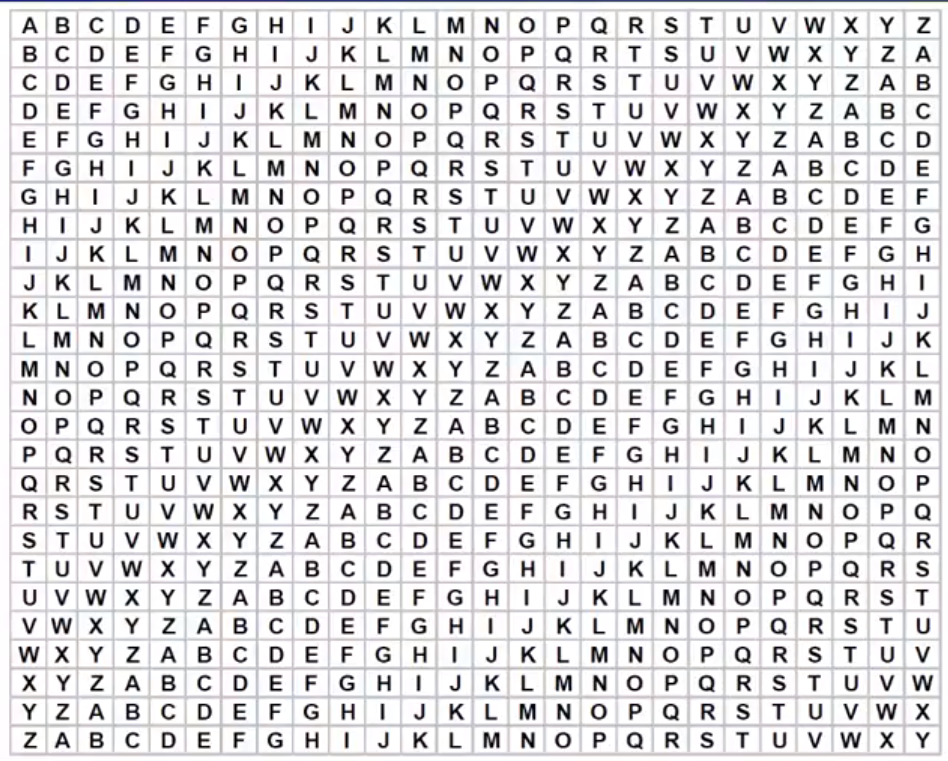
\includegraphics[width=0.8\linewidth]{immagini/img33}
\end{figure}

\begin{itemize}
	\item \textbf{Cifratura}: ogni paio di lettere di $m$ e $k$ individua una riga e una colonna, si prende il carattere che è contenuto nella cella a cui si riferiscono.
	Esempio: $m$: \texttt{PURPLE}, $k$: \texttt{CRYPTO}, $c$: \texttt{RLPEES}.
	Ad esempio il primo carattere sarà quello individuato dalla riga che inizia per \texttt{P} e la colonna che inizia con \texttt{C}.
	\item \textbf{Decifratura}: le stesse operazioni all'inverso.
	\item \textbf{Crittoanalisi}: la i-esima lettera di $m$ è cifrata come Cesare, la cui chiave è la i-esima lettera della chiave. Se la lunghezza della chiave è $l$, allora le lettere di $m$ in posizione $i$, $i+l$, $i+2l$... sono tutte cifrate con la stessa lettera di $k$.
	Ad esempio per $l = 5$, scrivo i caratteri del testo cifrato in righe lunghe $l$, quindi avrò (in termini di posizioni):
	\begin{equation*}
	\begin{matrix}
	1 & 2 & 3 & 4 & 5\\
	6 & 7 & 8 & 9 & 10\\
	11 & 12 & 13 & 14 & 15\\
	\vdots & \vdots & \vdots & \vdots & \vdots
	\end{matrix}
	\end{equation*}
	A questo punto ogni colonna è cifrata con la stessa chiave di Cesare, per cui si può effettuare un'analisi delle frequenze.
	Questo rompe il sistema anche se il numero delle chiavi è $26^5 = 11.881.376$.
	Come si trova però la lunghezza della chiave? Cerchiamo delle occorrenze di alcune sequenze, \texttt{PUXUL} + 15 lettere + \texttt{PUXUL}. La lunghezza della chiave potrebbe essere un divisore di 20.
\end{itemize}

\subsubsection*{Macchina Enigma}
Ci sono tre rotori (versione più semplice) ...

troppo lungo da spiegare 

\subsection*{DES}
\addcontentsline{toc}{subsection}{DES}
Negli anni 60-70 viene creato un crittosistema standard (casini fra banche ognuno aveva il suo ecc) da IBM, a partire dal vecchio Lucifer.
Nasce DES (Data Encryption Standard) che è un crittosistema simmetrico. (non è da sapere il funzionamento).
La lunghezza della chiave è di 56 bit, quindi ha $2^{56}$ possibili valori, il che lo rende oggi suscettibile da un attacco a forza bruta. Nella chiave vengono aggiungi bit di parità in posizioni 8, 16, 24, 32, ..., 64. (non ha senso, si mischia il livello crittografia e codifica).
L'algoritmo ha due fasi:
\begin{enumerate}
	\item Si generano le \textbf{chiavi derivate}: i bit della chiave vengono disposti in questo modo:
	\begin{figure}[h]
		\centering
		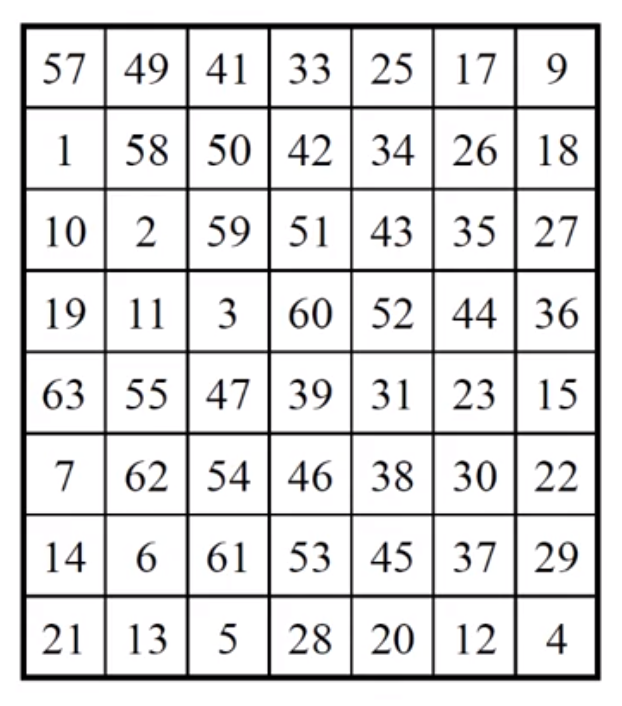
\includegraphics[width=0.5\linewidth]{immagini/img34}
	\end{figure}
	non è comodo, ma DES nasce per avere un'implementazione di tipo hardware...\\
	A questo punto divido in due blocchi: le prime quattro righe diventano il blocco $C_0$, le restanti quattro diventano $D_0$.
	A questo punto posso ottenere $C_1$ e $D_1$ ruotando verso sinistra i bit di $C_0$. In generale posso ottenere $C_n$ e $D_n$ a partire da $C_{n-1}$ e da $D_{n-1}$.
	Poi si selezionando alcune permutazioni e si generano le chiavi derivati $K_n$.
	Poi si divide il messaggio in chiaro in blocchi di 64 bit e comincia a fare scambi, xor, permutazioni ecc
\end{enumerate}
Proprietà DES:
\begin{itemize}
	\item Molto veloce (specialmente con hardware dedicato, le operazioni sono solo XOR, permutazioni, rotazioni, utilizzo di matrici di dimensioni fissate (lookup tables))
	\item La crittoanalisi di DES porta alla risoluzioni di equazioni non lineari (problemi simili al SAT, quindi NP-completi).
	\item Le S-boxes di DES (quelle della NSA e non quelle di Lucifer) resistono ad attacchi di crittoanalisi lineare e crittoanalisi differenziale.
	\item Quindi dal punto di vista matematico è ancora considerato sicuro, non più dal punto di vista informatico
	\item La chiave di 56 bit è troppo corta
	\item Esiste una macchina dedicata costruita con hardware di consumo (La DES Cracking Machine) che esplora l'intero spazio delle $2^{56}$ chiavi (1800 processori, trova la chiave segreta in due giorni).
\end{itemize}
A metà degli anni 90 una competizione internazionale fu organizzata per sostituire DES e creare un nuovo standard. Nel frattempo la comunità di crittografi consiglia di utilizzare il sistema 3DES:
\begin{enumerate}
	\item Si cifra $w$ usando $k_1$, ottenendo $c_1$,
	\item Si decifra $c_1$ usando $k_2$, ottenendo $c_2$,
	\item Si cifra $c_2$ usando $k_1$, ottenendo $c$
\end{enumerate}



